\section{Why GPUs?}


\subsection{Moore’s Law}


\par
Historically, computational demands have been predominantly linked to the Central Processing Unit (CPU), a complex component governing operations across diverse computing platforms, ranging from desktops to laptops and smartphones. The evolution of the modern CPU has been an intricate journey, driven in large part by the exacting standards set by the scientific and High Performance Computing (HPC) sectors. Transistors, the fundamental units of the CPU, dictate the performance of computers, mobile devices, and other contemporary electronic circuits.

\begin{figure}[!h]
\centering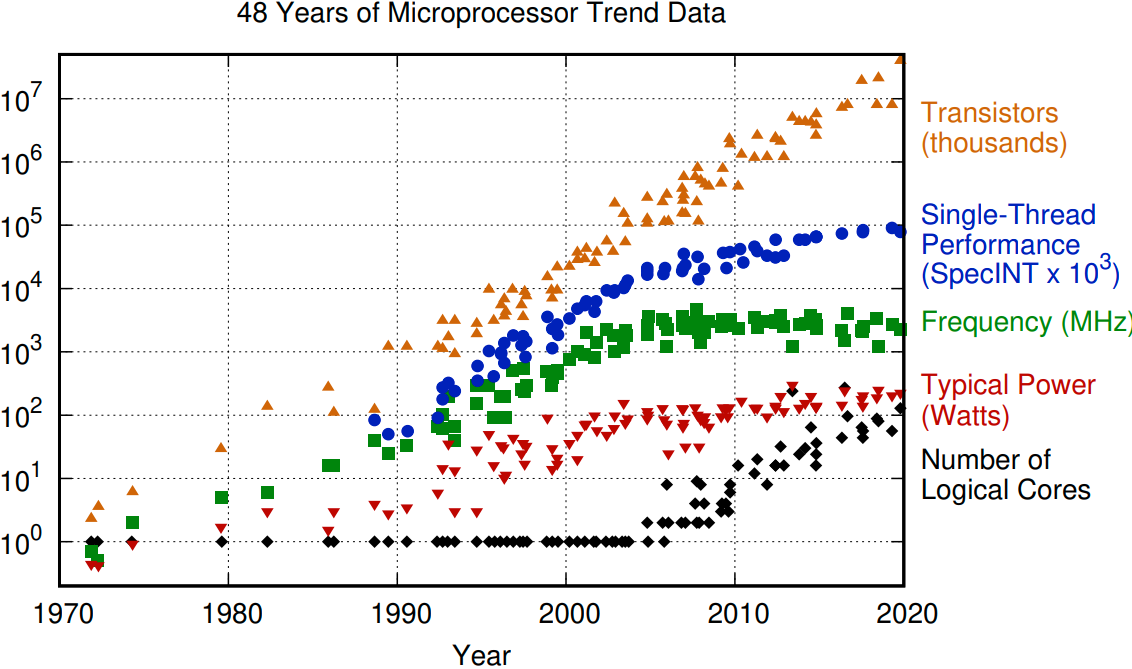
\includegraphics[width=0.8\textwidth]{fig_logo_history/microprocessor_trend.png}
\caption{The Moore’s Law timeline, including Moore's bend with transistors/CPU inflected with multi-core CPUs. Before 2000, the increase in the single core clock frequency was the major source of the increase in the performance. Mid 2000 mark a transition towards multi-core processors. Original data up to the year 2010 collected and plotted by M. Horowitz, F. Labonte, O. Shacham, K. Olukotun, L. Hammond, and C. Batten. New plot and data collected for 2010-2019 by K. Rupp~\cite{microprocessor-trend-data}. }\label{fig:microprocessor_trend}
\end{figure}


\par
\textbf{The Moore's Law} states that the number of transistors in a dense integrated circuit doubles about every two years (Fig.~\ref{fig:microprocessor_trend}).
More transistors means smaller size of a single element, so higher core frequency can be achieved.
Up until the year 2000s, the CPU manufacturers including IBM, Intel, and AMD produce faster CPUs by making them work at a higher speed, 16 MHz, 20 MHz, 66 MHz, 100 MHz, and eventually 200, 333, 466 MHz$\cdots$.
It looks like they could keep increasing the CPU speeds and provide higher performance every year.
However, at the beginning of 2000s, it was obvious that continuously increasing the CPU speeds couldn’t go on forever due to the power consumption limits.
The power consumption scales with frequency to the third power, and therefore the growth in the core frequency has slowed down significantly, which limits the improvement on the computational performance of single-core CPUs.


\par
Increasing computational performance of processing units has been sustained with two main strategies over the years: 1) Increase the single processor performance; and 2) More recently, increase the number of physical cores.
Both strategies promote the development of parallel computing for scientific and HPC community.
In fact, higher performance of a single node has to rely on its more complicated structure and still can be achieved with SIMD (single instruction multiple data), branch prediction, $etc$.


% -------------------------------------------------------------------- %


\subsection{Parallel computing}


\par
Parallel computing, which is interchangeable with parallel processing or in conjunction with parallel programming, refers to the process of decomposing a computational problem into smaller subtasks that can be executed simultaneously using multiple processing units (Fig.~\ref{fig:comput_serial_parallel}).
Parallel computing is critical for large scale projects in which speed and accuracy are needed.
It is a complex task, but allows developers, researchers, and users to accomplish research and analysis quicker than with a program that can only process one task at a time.


\begin{figure}[!h]
\centering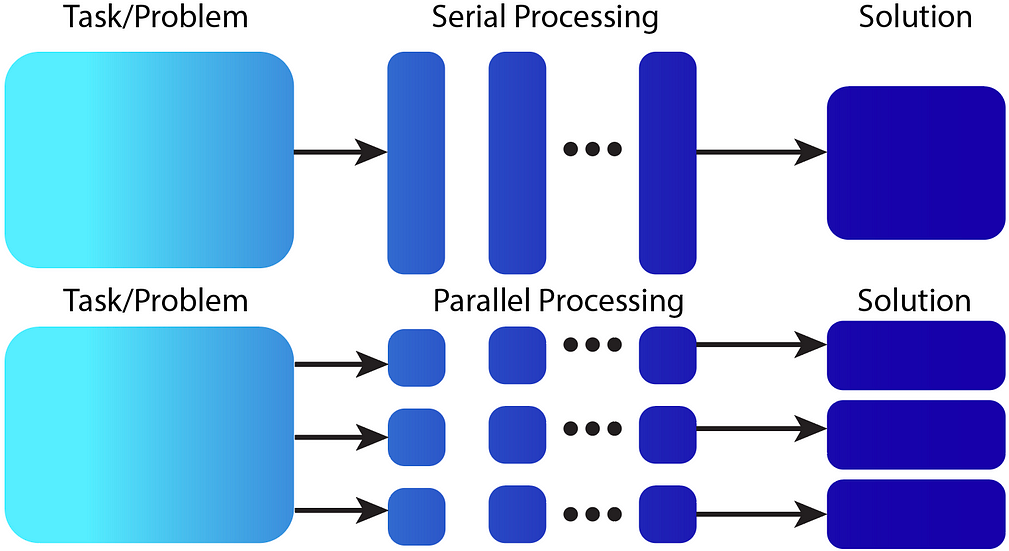
\includegraphics[width=0.8\textwidth]{fig_logo_history/comput_serial_parallel.png}
\caption{Serial processing and parallel computing.}\label{fig:comput_serial_parallel}
\end{figure}


\par
How a problem is split into smaller subtasks strongly depends on the problem.
There are two fundamental types of parallelism in applications:~\textbf{task parallelism} and~\textbf{data parallelism}.
\begin{itemize}
    \item Task parallelism arises when there are many tasks or functions that can be operated independently and largely in parallel. Task parallelism focuses on distributing functions across multiple cores.
    \item Data parallelism arises when there are many data items that can be operated on at the same time. Data parallelism focuses on distributing the data across multiple cores.
\end{itemize}


\par
More pertinently, two of the most commonly used programming approaches are SIMD and MIMD.
SIMD, or single instruction multiple data, is a form of parallel computing related to a computer architecture.
There are multiple cores in the computer.
All cores execute the same instruction stream at any time, each operating on different data streams.
SIMD is typically used to analyze large data sets that are based on the same specified benchmarks.
Vector computers are typically characterized as SIMD, and most modern computers employ a SIMD architecture.
Perhaps the biggest advantage of SIMD is that, while writing code on the CPU, the programmers can continue to think sequentially yet achieve parallel speed-up from parallel data operations because the compiler takes care of the details.
MIMD, or multiple instruction multiple data, is another common form of parallel computing and computer architecture in which multiple cores operate on multiple data streams, each executing independent instructions.
Many MIMD architectures also include SIMD execution sub-components.


\par
Besides SIMD and MIMD, the computer architecture can also be subdivided by its memory organization, which is generally classified into two types:~\textbf{multi-node with distributed memory} and~\textbf{multiprocessor with shared memory}.
In a multi-node system, large scale computational engines are constructed from many processors connected by a network. Each processor has its own local memory, and processors can communicate the contents of their local memory over the network.
The left figure in Fig.~\ref{fig:multinode_vs_multicore} shows a typical multi-node system with distributed memory. These systems are often referred to as~\textbf{clusters}.
Multiprocessor architectures typically range in size from dual-processor to dozens or hundreds of processors. These processors are either physically connected to the same memory (the right figure in Fig.~\ref{fig:multinode_vs_multicore}), or share a low-latency link (such as PCI-Express or PCIe).
Although sharing memory implies a shared address space, it does not necessarily mean there is a single physical memory.
Such multiprocessors include both single-chip systems with multiple cores, known as~\textbf{multicore}, and computers consisting of multiple chips, each of which might have a multicore design.
Multicore architectures have displaced single-core architectures permanently. The term~\textbf{many-core} is usually used to describe multicore architectures with an especially high number of cores (tens or hundreds).
Recently, computer architectures have been transitioning from multicore to many-core, and a representative of many-core computing hardware is graphics processing unit (GPU).


\begin{figure}[!h]
\centering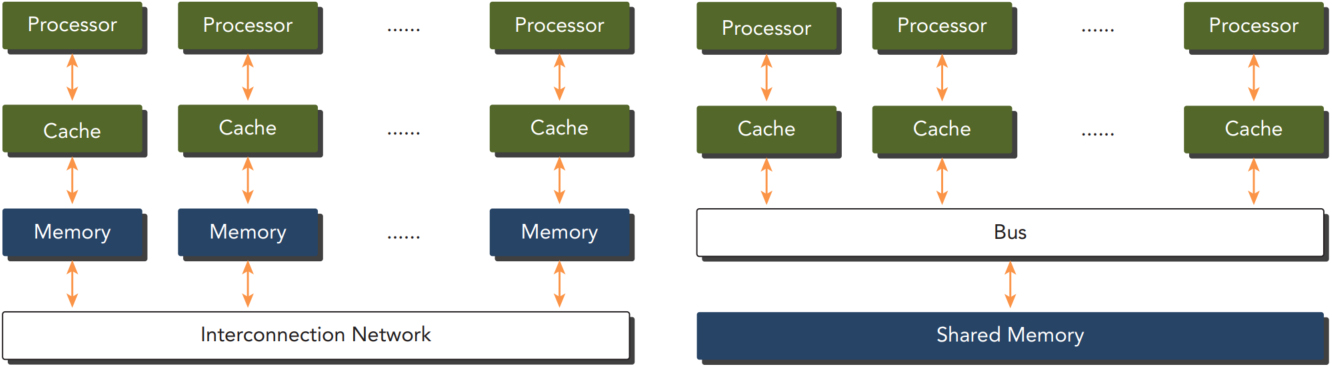
\includegraphics[width=0.9\textwidth]{fig_hardware/multinode_vs_multicore.jpg}
\caption{Two types of computer architectures depending on their memory organization. Left for multi-node with distributed memory and right for multiprocessor with shared memory.}\label{fig:multinode_vs_multicore}
\end{figure}


% -------------------------------------------------------------------- %


\subsection{Graphics processing units}


\par
A GPU is a specialized electronic circuit initially designed to accelerate computer graphics and image processing (either on a video card or embedded on the motherboards, mobile phones, personal computers, workstations, and game consoles), but have recently been evolved to be powerful, general-purpose, fully programmable, task and data parallel processors, ideally suited to tackle massively parallel computing problems due to their many-core architectures~\cite{gpu_wiki}.


% -------------------------------------------------------------------- %


\subsection{Advantages and limitations of CPU and GPU programming}


\par
CPUs have several distinct advantages for modern computing tasks:
\begin{itemize}
    \item Flexibility: a CPU is a general-purpose processor that can handle many tasks, and multitask between multiple activities.
    \item Faster in many contexts: CPUs are faster than GPUs when handling operations like data processing in RAM, I/O operations, and operating system administration.
    \item Precision: CPUs can support mid-range math operations with higher precision than GPUs, which is important for many use cases.
    \item Cache memory: CPUs have a large local cache memory, which lets them handle large sets of linear instructions.
    \item Hardware compatibility: CPUs are compatible with all types of motherboards and system designs, whereas GPUs require specialized hardware support.
\end{itemize}


CPUs have the following disadvantages compared to GPUs:
\begin{itemize}
    \item Parallel processing: CPUs are less adept at tasks that require millions of identical operations because of their limited parallelism.
    \item Slower development: CPUs are a very mature technology that is already reaching the limits of its development, while GPUs have much more potential to improve.
    \item Compatibility: several types of CPUs, including x86 and ARM processors, and software may not be compatible with all types.
\end{itemize}


The unique advantages of GPUs include:
\begin{itemize}
    \item High data throughput: a GPU can perform the same operation on many data points in parallel, so that it can process large data volumes at speeds unmatched by CPUs.
    \item Massive parallelism: a GPU has hundreds of cores, allowing it to perform massively parallel calculations, such as matrix multiplications.
    \item Suitable for specialized use cases: GPUs can provide massive acceleration for specialized tasks like deep learning, big data analytics, genomic sequencing, and more.
    \item Improved energy efficiency: Compared to CPUs, GPUs can perform more calculations per watt of power consumed, which can result in significant energy savings. This is indeed evident from the Green500 list~\cite{green500}.
    \item Cost-effectiveness: GPUs can be more cost-effective than traditional CPU-based systems for certain workloads.
\end{itemize}


The limitations of GPUs compared to CPUs include:
\begin{itemize}
    \item Difficulty handling complexity: Not all workloads can be efficiently parallelized and accelerated on GPUs. A GPU can struggle with processing tasks that are not well structured. They cannot efficiently process branching logic, sequential operations, or other complex programming patterns. % Certain types of workloads, such as those with irregular data access patterns or high branching behavior, may not see significant performance improvements on GPUs.
    \item Steeper learning curve: Depending on the GPU programming API that you choose, GPU computing could require specialized skills in GPU programming and knowledge of GPU architecture, leading to a steeper learning curve compared to CPU programming. Fortunately, if you study this training material closely you will become productive with GPU programming quickly!
\end{itemize}


\par
GPU computing is not meant to replace CPU computing.
Each approach has advantages for certain kinds of programs.
CPU computing is good for control-intensive tasks, and GPU computing is good for data-parallel computation-intensive tasks.
When CPUs are complemented by GPUs, it makes for a powerful combination.
The CPU is optimized for dynamic workloads marked by short sequences of computational operations and unpredictable control flow; and GPUs aim at the other end of the spectrum: workloads that are dominated by computational tasks with simple control flow. 


\par
If a problem has a small data size, sophisticated control logic, and/or low-level parallelism, the CPU is a good choice because of its ability to handle complex logic and instruction-level parallelism.
If the problem at hand instead processes a huge amount of data and exhibits massive data parallelism, the GPU is the right choice because it has a large number of programmable cores, can support massive multi-threading, and has a larger peak bandwidth compared to the CPU.
The CPU + GPU heterogeneous parallel computing architectures evolved as such a combination ensures that the characteristics of the GPU and CPU complement each other, leading to a full utilization of the computational power of the combined CPU + GPU system.


\par
For the heterogeneous architecture, CPUs and GPUs are discrete processing components connected by the PCI-Express bus (Fig.~\ref{fig:cpu_gpu_architecture}).
The switch from traditional homogeneous CPU systems to current heterogeneous CPU+GPU systems is a milestone in the history of HPC.
\textbf{Homogeneous computing} uses one or more processor of the same architecture to execute an application.
\textbf{Heterogeneous computing} instead uses a suite of processor architectures to execute an application, applying tasks to architectures to which they are well-suited, yielding performance improvement as a result.


\begin{figure}[htbp]
\centering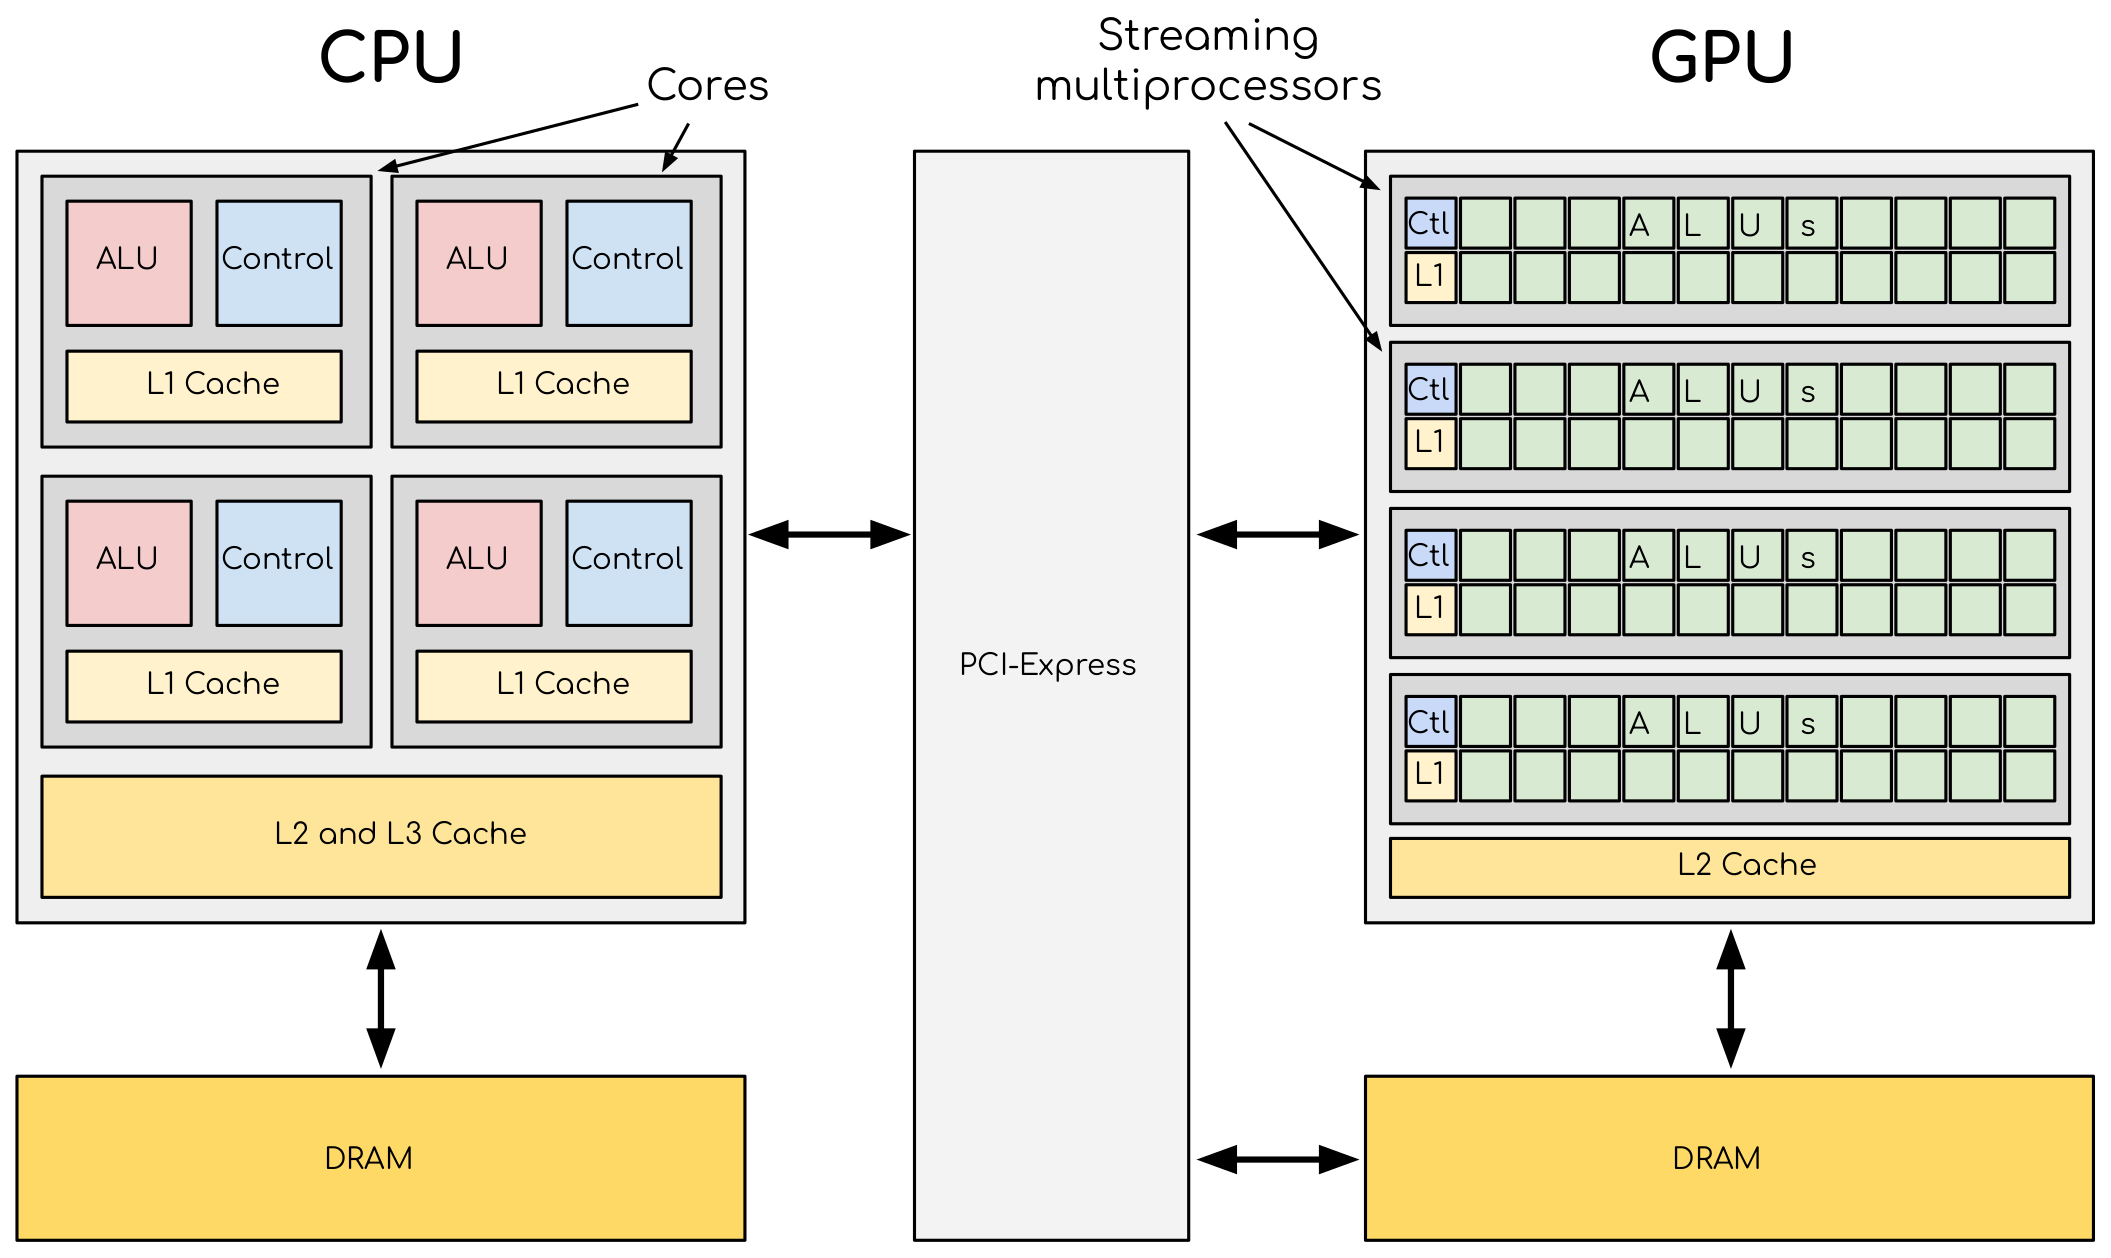
\includegraphics[width=0.8\textwidth]{fig_hardware/cpu_gpu_architecture.png}
\caption{A comparison of CPU and GPU architecture. CPU (left) has complex core structure and pack several cores on a single chip. GPU cores are very simple in comparison, they also share data and control between each other. This allows to pack more cores on a single chip, thus achieving very high compute density.}\label{fig:cpu_gpu_architecture}
\end{figure}


\par
The GPU-enabled heterogeneous computing systems require a heterogeneous programming model that involves both CPU and GPU, where the CPU and its memory are referred to as the~\textbf{host}, and the GPU and its memory as the~\textbf{device}.
Correspondingly, a program running on heterogeneous computing systems consists of two parts, the host code running on CPUs and the device code running on GPUs.
The program executing on a heterogeneous platform is typically initialized by the CPU.
The CPU code is responsible for managing the environment, code, and data for the device before loading compute-intensive tasks on the device.
With computational intensive applications, program sections often exhibit a rich amount of data parallelism. GPUs are used to accelerate the execution of this portion of data parallelism.
Therefore, for optimal performance we need to use both CPU and GPU for computational intensive applications, executing the sequential parts or task parallel parts on the CPU and intensive data parallel parts on the GPU.


\par
To support joint CPU + GPU execution of an application, the three major GPU vendors, NVIDIA, AMD, and Intel, in addition to design and produce GPUs for HPC, have designed their own computing platforms~\textbf{CUDA} (Compute Unified Device Architecture),~\textbf{ROCm} (Radeon Open Compute), and~\textbf{oneAPI}, respectively.
This way they can offer optimization, differentiation (offering unique features tailored to their devices), vendor lock-in, licensing, and royalty fees, which can result in better performance, profitability, and customer loyalty.
There are also cross-platform APIs (application programming interfaces) such~\textbf{DirectCompute} (only for Windows operating system),~\textbf{OpenCL}, and~\textbf{SYCL}.
These are the main topics of this workshop targeted for GPU programming.


% -------------------------------------------------------------------- %


\subsection{The Top500 HPC supercomputers at a glance}


\par
HPC is a set of technologies that enable large-scale, massively parallel computing.
Traditionally, HPC systems were based on CPUs, but modern HPC systems increasingly make use of GPUs.
It is common for HPC servers to combine multiple CPUs and GPUs in one system.


\par
The TOP500 project ranks and details the 500 most powerful non-distributed HPC systems in the world.
This project was launched in 1993 to improve and renew the Mannheim supercomputer statistics, and publishes an updated list of the supercomputers twice a year~\cite{top500_1}.
Fig.~\ref{fig:supercomputer_top5} shows the top-5 HPC systems as of June 2023~\cite{top500_2}, where the columns show:
\begin{itemize}
    \item Cores: Number of processors
    \item Rmax: Maximal LINPACK performance achieved
    \item Rpeak: Theoretical peak performance
    \item Power: Power consumption
\end{itemize}


\begin{figure}[htbp]
\centering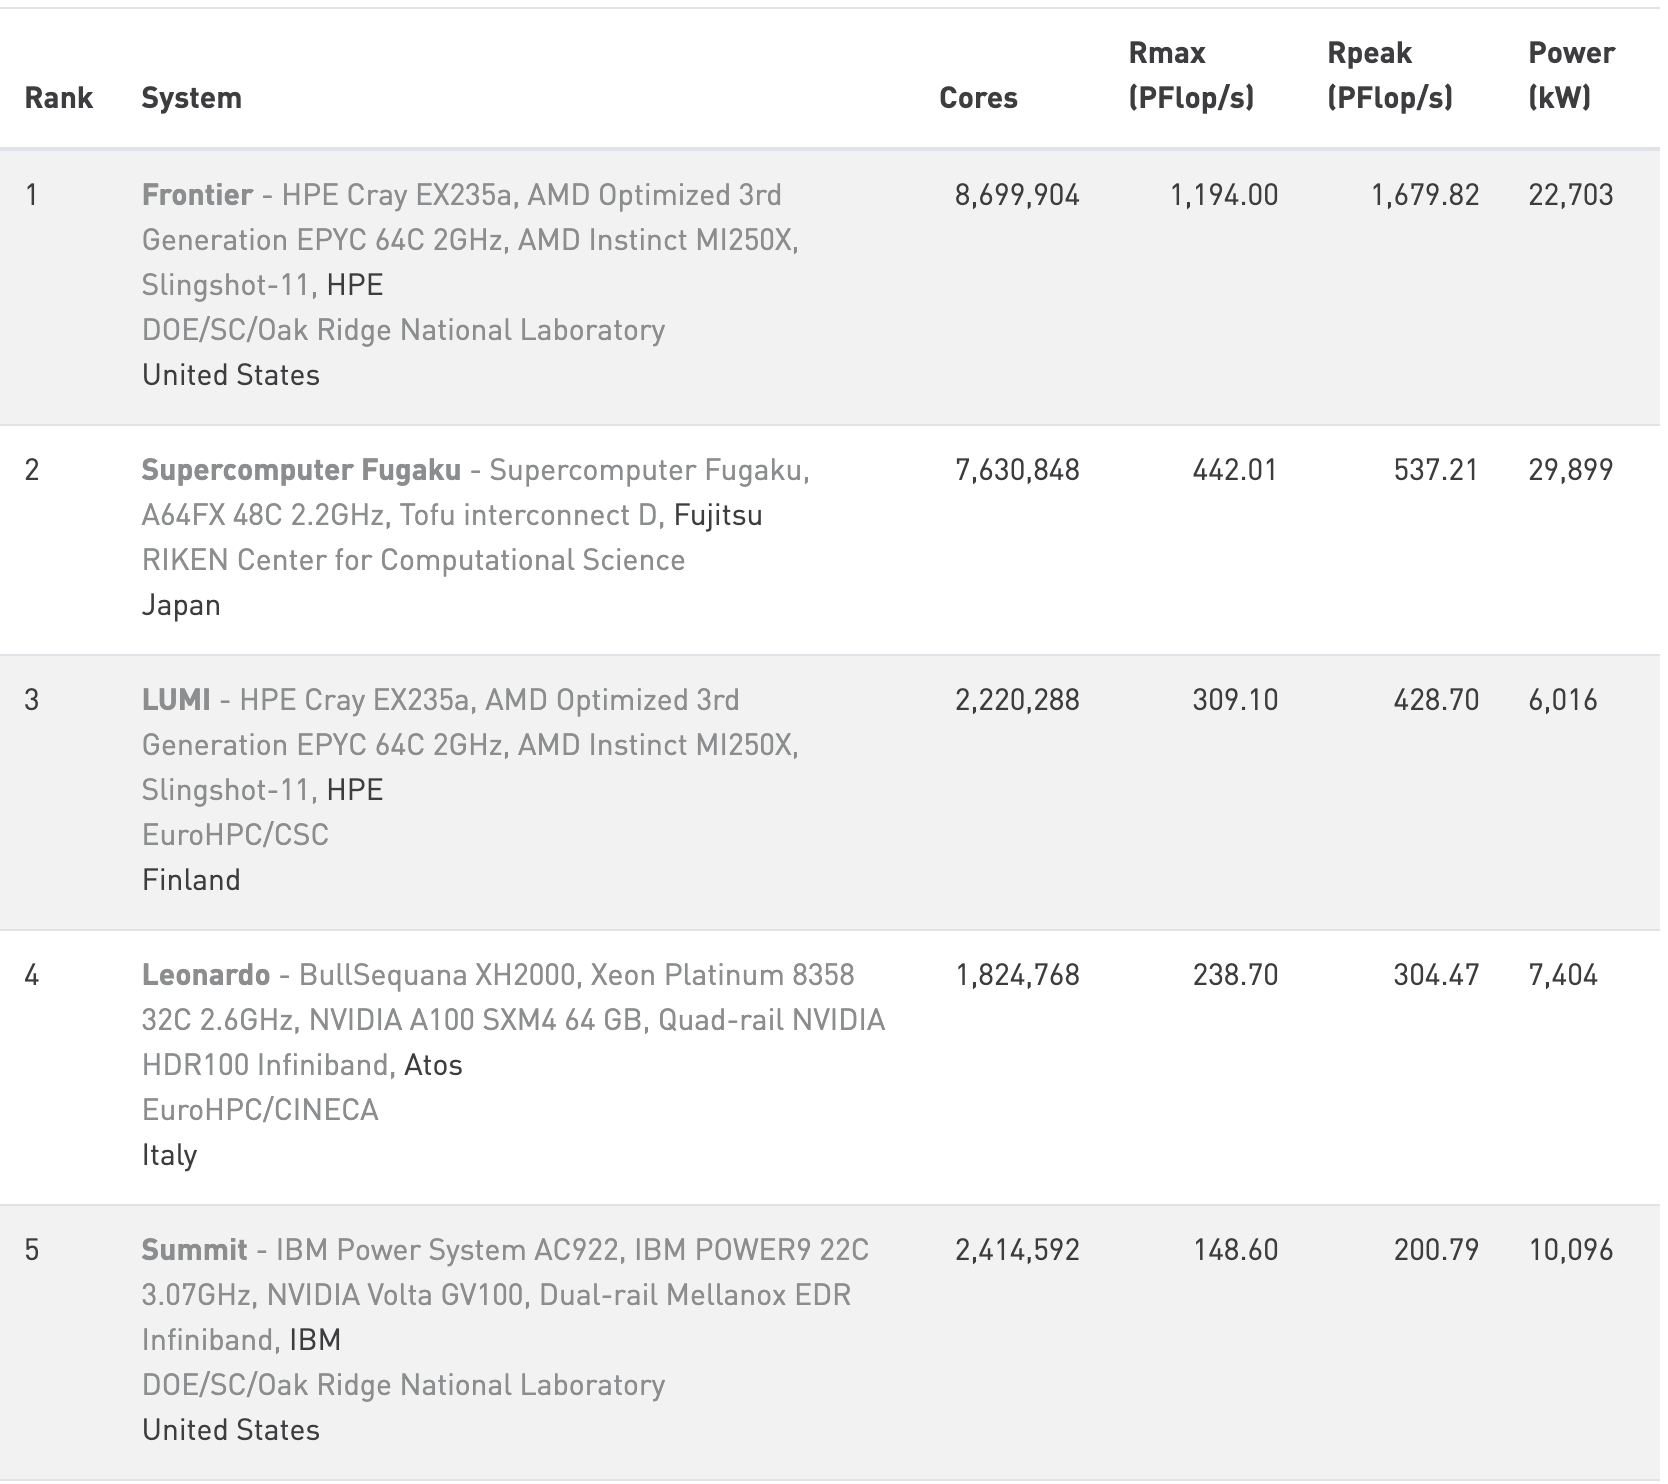
\includegraphics[width=0.8\textwidth]{fig_logo_history/supercomputer_top5.png}
\caption{The top 5 HPC systems on the Top500 list from June, 2023.}\label{fig:supercomputer_top5}
\end{figure}


\par
All systems in the top-5 positions contain GPUs from AMD or NVIDIA, except for the Fugaku system at the RIKEN Center for Computational Science in Kobe, Japan, which instead relies on custom-built Arm A64FX CPUs.
The Frontier system at the Oak Ridge National Laboratory, Tennessee, USA remains the No. 1 system on the TOP500 and is still the only system reported with an HPL performance exceeding one Exaflop/s.
Frontier is based on the latest HPE Cray EX235a architecture and equipped with AMD EPYC 64C 2GHz processors. The system has 8,699,904 total cores, a power efficiency rating of 52.59 gigaflops/watt, and relies on Slingshot-11 interconnect for data transfer.  
The No. 3 and No. 4 HPC systems are the LUMI system at EuroHPC/CSC in Finland and the Leonardo system at EuroHPC/CINECA in Italy, and have HPL scores of 309.1 Pflop/s and 239 Pflop/s, respectively.
The Summit system, also at the Oak Ridge National Laboratory, Tennessee, USA, was launched in 2018 and has a hybrid architecture with each node containing multiple IBM POWER9 CPUs and NVIDIA Volta GPUs all connected together with NVIDIA’s high-speed NVLink.
Each node has over half a terabyte of coherent memory (high bandwidth memory + DDR4) addressable by all CPUs and GPUs plus 800GB of non-volatile RAM that can be used as a burst buffer or as extended memory.

